
Para la problemática presentada anteriormente presentamos en esta sección: el objetivo, objetivos específicos, la justificación, el alcance y la descripción de la propuesta de solución.\\

%La realización de la propuesta está basada en el siguiente objetivo.\\
%Pues comienzas haciendo referencia a la imagen y dando una breve explicación de lo que contiene
%"En la imagen x podemos observar de una forma más precisa...
\section{Objetivo}

Para mitigar las causas y reducir el impacto de los problemas que se tienen nos basamos en el siguiente objetivo: \\

Desarrollar e implementar una aplicación web para el apoyo en el control de la correspondencia.\\

\subsection{Objetivos Específicos}

\begin{itemize}
	\item Cubrir los lineamientos establecidos para el control de correspondencia en el Manual de Procedimientos del CMPL.
	\item Tener un respaldo electrónico de los oficios y memorándums para posterior consulta.
	\item Llevar un registro de los oficios entrantes y salientes.
	\item Notificar al personal que tiene correspondencia por atender.
	\item Dar seguimiento a los asuntos que se deben atender.
\end{itemize}

%\section{Justificación}
%De acuerdo con los objetivos anteriores 
%Desarrollar e implementar una aplicación web que fortalezca los procesos de la administración del CMPL.

\section{Alcance}

Para visualizar de una mejor manera el alcance de la aplicación se divide de la siguiente manera: \\

\begin{itemize}
	\item Funcionalidad: muestra los módulos por los que estará formado la aplicación y los diferentes tipos de usuarios que la utilizarán.
	\item Plataforma: el hardware, el software y los servicios necesarios para la aplicación.
	\item Procedimiento: descripción y mejoras al procedimiento anterior.
	\item Información: la información que se va a manejar dentro de la aplicación.
	\item Propiedades de software: son los atributos con los que contará la aplicación.
	\item Interacción con el usuario: la forma en que el usuario podrá hacer el intercambio de información con la aplicación.
\end{itemize}

%%%%%%%%%% FUNCIONALIDAD %%%%%%%%%%%%
%%%%%%%%%%%%%%%%%%%%%%%%%%%%%%%%%%%%%

\subsection{Funcionalidad}

Con base en los objetivos anteriores la aplicación estará conformada por 5 módulos y 6 tipos de usuarios. En la figura x se observa de manera más precisa como estará formada. \\ 

	\begin{figure}[htbp!]
		\centering
			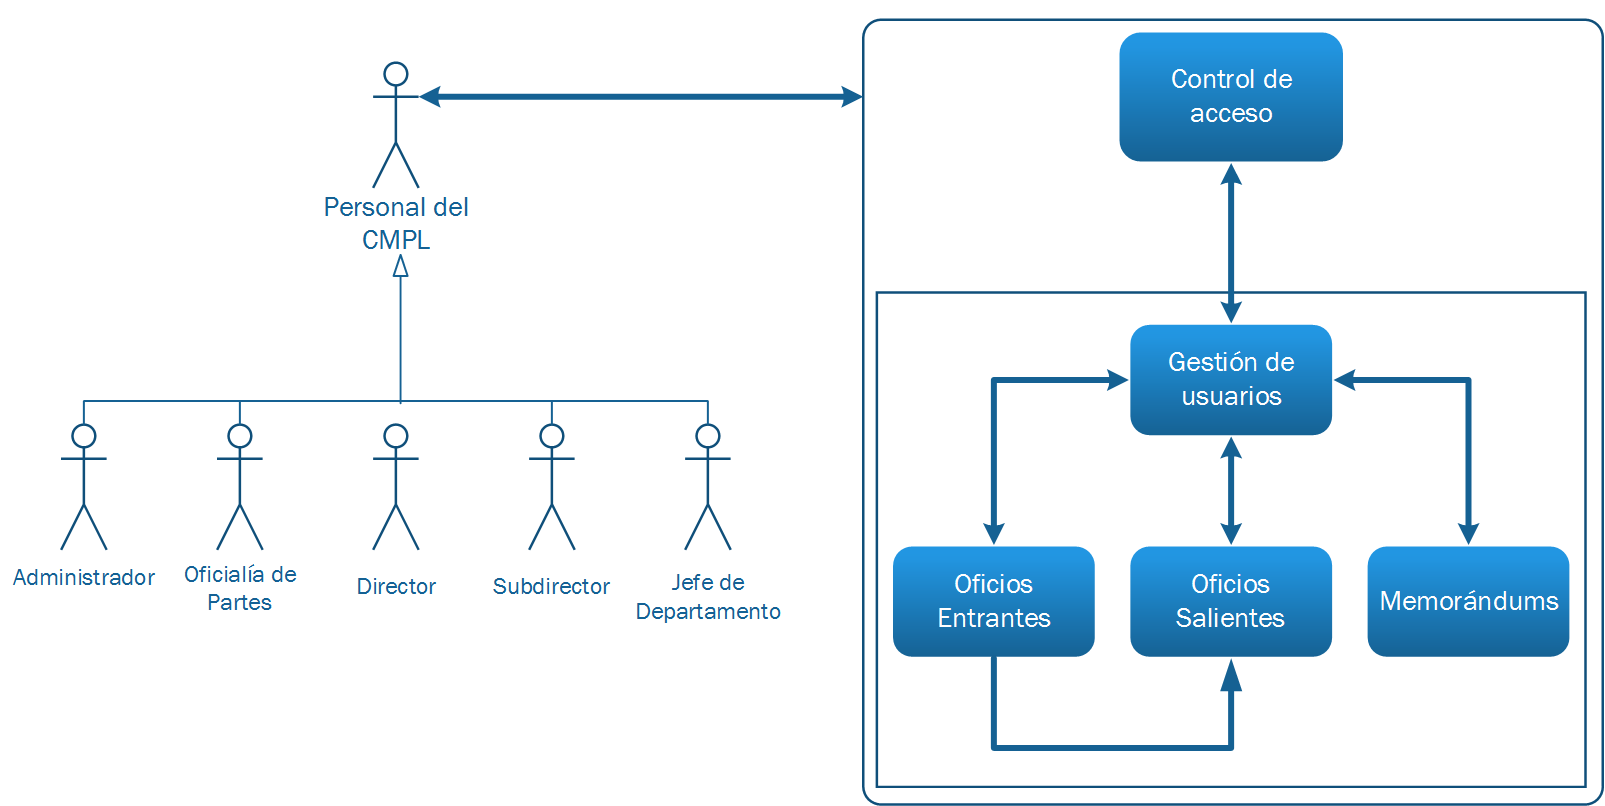
\includegraphics[width=0.8\textwidth]{images/propuesta/diagramabloques}
		\caption{Diagrama de Bloques de la Aplicación.}
	\end{figure}

\subsubsection{Descripción de Módulos}
\subsubsection{Control de acceso}

Este módulo servirá para restringir el acceso a usuarios dentro de la aplicación para que cada uno pueda acceder a todas sus funciones de acuerdo del tipo de usuario que sea.\\ %Cuenta con una pantalla que tiene un formulario de autenticación donde se le solicita al usuario su correo institucional y su contraseña. Cuando el usuario ingresa sus credenciales la aplicación verifica su correo y su contraseña; si existen entonces la aplicación muestra la pantalla principal de acuerdo al tipo de usuario que sea. En caso contrario, la aplicación regresa a la pantalla de autenticación con un mensaje de error diciendo que los datos introducidos no son válidos.\\

\subsubsection{Gestión de usuarios}
En este módulo se encontrará alojada la información del personal del CMPL que tendrá acceso a la aplicación, que son el personal administrativo y de apoyo. Se podrán modificar los datos del personal, así como agregar y dar de baja usuarios. \\ %la información almacenada del personal del CMPL en este módulo es: nombre, apellido paterno, apellido materno, nivel de estudios, departamento al que pertenece, extensión, correo institucional y contraseña. Sirve para mostrar una pantalla con el directorio interno del CMPL, modificar los datos del personal, incluyendo la contraseña.\\

\subsubsection{Correspondencia (Oficios y Memorándums)}
Este módulo tendrá las pantallas de registro de correspondencia de oficios entrantes y salientes, así como los memorándums.\\ %con un formulario que contiene los siguientes campos: número de oficio, fecha de redacción, área que emite, emisor, cargo del emisor, destinatario, cargo del destinatario, dependencia, asunto, fecha de acuse, nombre de quien entrega y si requiere o no respuesta. También cuenta con un selector de archivos que permite la carga del documento escaneado en formato PDF y adjuntarlo al registro. Tiene, además, una pantalla donde se pueden consultar todos los oficios y memorándums enviados y recibidos, por ID, asunto, emisor, cargos de emisor, fecha de recibido, fecha de acuse, dependencia que emite, nombre de quien entrega, pendientes, en espera o un concentrado de todos los oficios y todos los memorándums.\\

En cuanto a los tipos de usuarios que utilizarán la aplicación, cada uno tiene responsabilidades diferentes en el CMPL por lo tanto dentro de la aplicación sus funciones serán diferentes y se describen a continuacion: \\
%%%%%%%%%%%%%%%%%%%%%%%%%%%%%%%%%%%%%%%%%%%%%
%%%%%%%%%%%%%%%%%ROLES DE USUARIOS%%%%%%%%%%%
\subsubsection{Descripción de roles de usuarios}

\subsubsection{Administrador}
Es el jefe del Departamento de Sistemas y Banco de Datos del CMPL. Tiene el control total de la administración de la información mostrada en la aplicación web.\\

\textbf{Responsabilidades:}
\begin{itemize}
	\item Dar de alta nuevos usuarios.
	\item Editar usuarios existentes.
	\item Eliminar usuarios.
	\item Registrar correspondencia saliente (oficios y memorándums).
	\item Consultar correspondencia.
	\item Dar seguimiento a su correspondencia.
\end{itemize}

\subsubsection{Oficialía de Partes}
Es la persona que lleva a cabo la recepción de correspondencia formal del CMPL. Recibe los documentos de correspondencia y los registra en una bitácora; firma y sella de recibido y turna los oficios y memos a sus respectivos destinatarios.\\

\textbf{Responsabilidades:}
\begin{itemize}
	\item Verificar que los documentos recibidos cumplan con todos los lineamientos requeridos para su recepción.
	\item Registrar la correspondencia formal interna y externa del CMPL.
	\item Turnar los oficios y memorándums a sus respectivos destinatarios.
	\item Registrar correspondencia saliente.
\end{itemize}

\subsubsection{Personal CMPL}
Es un trabajador del CMPL registrado en el directorio, que no es Jefe del Departamento de Sistemas y Banco de Datos o encargado de Oficialía de Partes.\\

\textbf{Responsabilidades:}
\begin{itemize}
	\item Checar su correspondencia entrante.
	\item Registrar correspondencia saliente.
	\item Turnar correspondencia.
	\item Recibir correspondencia.
	\item Atender observaciones a los oficios registrados.
\end{itemize}

\subsubsection{Director}
Es un trabajador del CMPL con el nombramiento de “Director”. Es la persona que representa al centro ante otras dependencias. Se encarga de administrar y gestionar las decisiones importantes del centro junto con su grupo de trabajadores.\\

\textbf{Responsabilidades:}
\begin{itemize}
	\item Turnar oficios entrantes.
	\item Turnar copia de oficios entrantes.
	\item Firmar oficios salientes.
	\item Cancelar proceso de oficios entrantes.
	\item Cancelar proceso de oficios salientes.
	\item Ver detalles de correspondencia.
	\item Responder oficios.
\end{itemize}

\subsubsection{Jefe de Departamento}
Es un trabajador del CMPL que está como encargado de alguna de las diferentes jefaturas que existen en el centro. Se encarga de apoyar a la dirección con las decisiones importantes para el CMPL y de atender los asuntos que conciernen con el departamento del cual está encargado.\\

\textbf{Responsabilidades:}
\begin{itemize}
	\item Atender correspondencia a nombre del director.
	\item Manejar los indicadores mensuales.
	\item Cancelar proceso de correspondencia saliente.
	\item Generar oficios salientes nuevos.
	\item Dar respuesta a oficios entrantes.
	\item Atender observaciones a los oficios registrados.
\end{itemize}

\subsubsection{Subdirector}
Es un trabajador del CMPL que esta como encargado en alguna de las subdirecciones existentes dentro del centro. Se encarga de las decisiones que conciernen al área y de la administración de dicho departamento. Puede que tenga a su cargo otra jefatura y debe trabajar en conjunto con esta otra área.\\ 

\textbf{Responsabilidades:}
\begin{itemize}
	\item Responder oficios entrantes.
	\item Registrar oficios salientes.
	\item Turnar correspondencia en caso de que tenga alguna jefatura a su cargo.
	\item Ver detalles de correspondencia.
	\item Atender observaciones a los oficios registrados.
\end{itemize}

%%%%%%%%%% PLATAFORMA %%%%%%%%%%%%%%%
%%%%%%%%%%%%%%%%%%%%%%%%%%%%%%%%%%%%%
\subsection{Plataforma}

	\begin{figure}[htbp!]
		\centering
			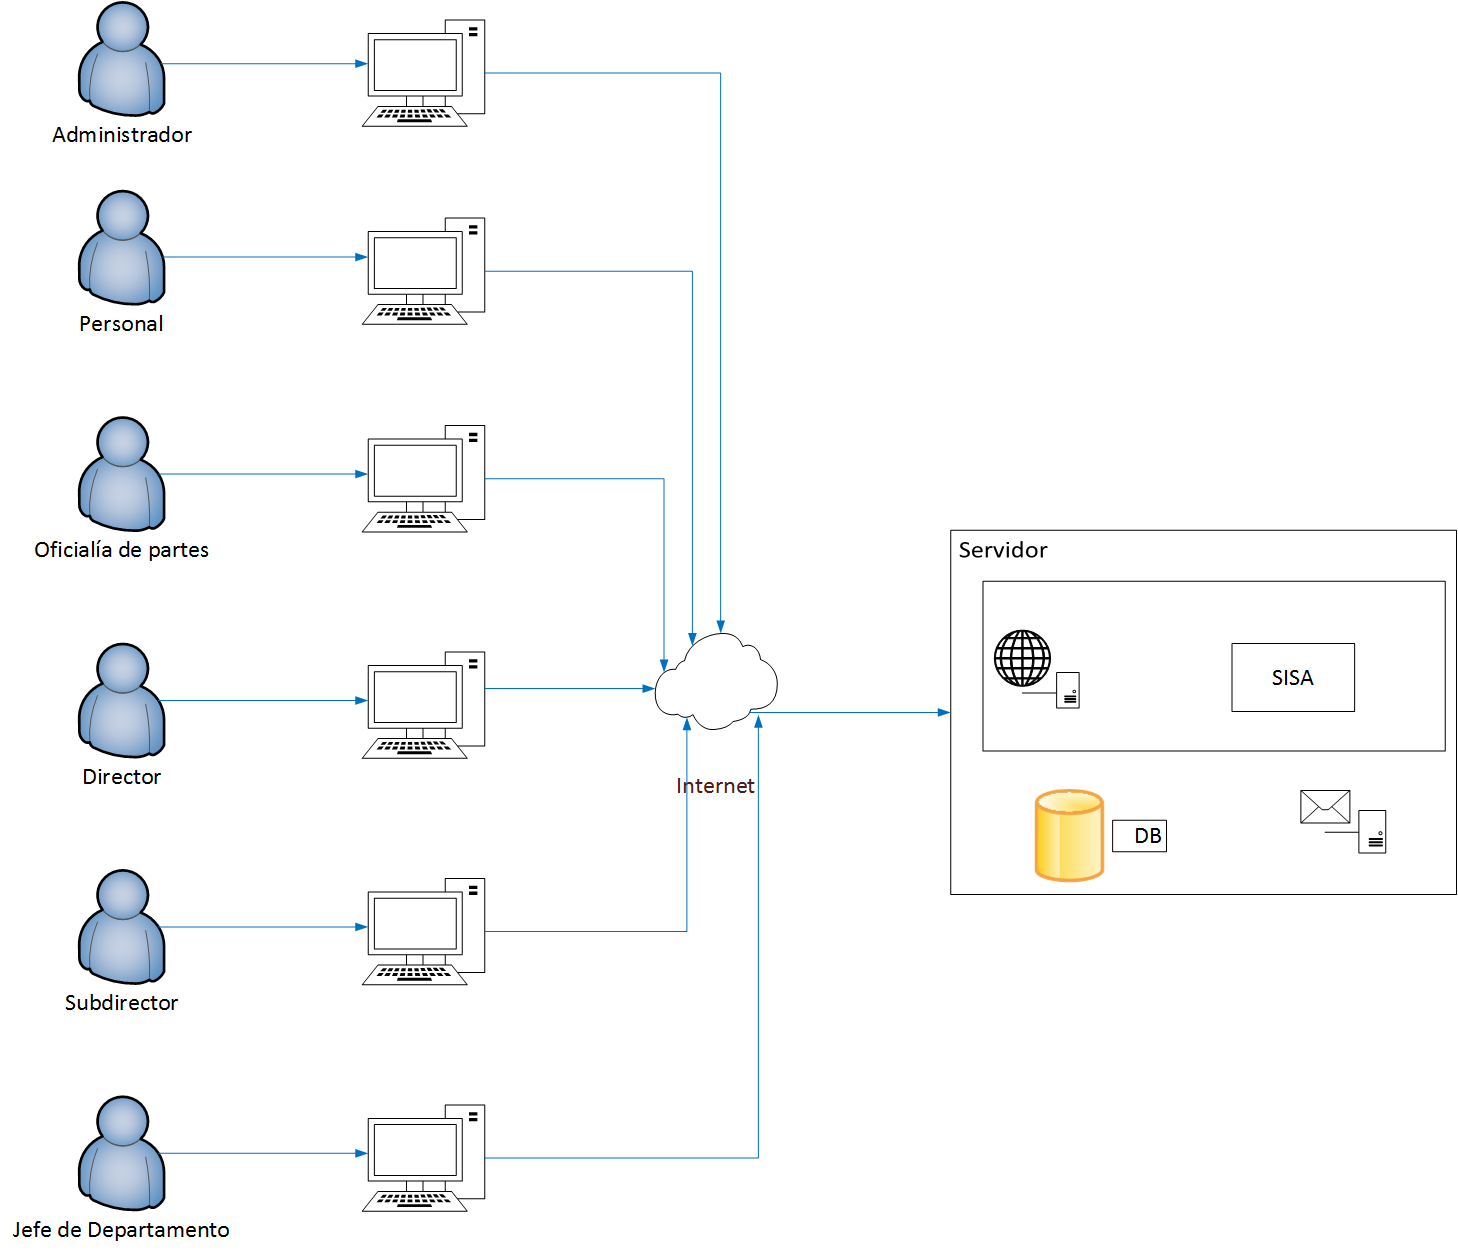
\includegraphics[width=0.8\textwidth]{images/propuesta/arquitectura}
		\caption{Arquitectura de la Aplicación.}
	\end{figure}
	
%%%%%%%%%% PROCEDIMIENTO %%%%%%%%%%%%
%%%%%%%%%%%%%%%%%%%%%%%%%%%%%%%%%%%%%
\subsection{Procedimiento}

%%%%%%%%%% INFORMACION %%%%%%%%%%%%%%
%%%%%%%%%%%%%%%%%%%%%%%%%%%%%%%%%%%%%
\subsection{Información}

%%%%%%%%%% PROPIEDADES DE SW %%%%%%%%
%%%%%%%%%%%%%%%%%%%%%%%%%%%%%%%%%%%%%
\subsection{Propiedades de software}

%%%% INTERACCION CON EL USUARIO %%%%%
%%%%%%%%%%%%%%%%%%%%%%%%%%%%%%%%%%%%%
\subsection{Interacción con el usuario}
Cuenta con una pantalla que tiene un formulario de autenticación donde se le solicita al usuario su correo institucional y su contraseña. Cuando el usuario ingresa sus credenciales la aplicación verifica su correo y su contraseña; si existen entonces la aplicación muestra la pantalla principal de acuerdo al tipo de usuario que sea. En caso contrario, la aplicación regresa a la pantalla de autenticación con un mensaje de error diciendo que los datos introducidos no son válidos.

la información almacenada del personal del CMPL en este módulo es: nombre, apellido paterno, apellido materno, nivel de estudios, departamento al que pertenece, extensión, correo institucional y contraseña. Sirve para mostrar una pantalla con el directorio interno del CMPL, modificar los datos del personal, incluyendo la contraseña.\\

%con un formulario que contiene los siguientes campos: número de oficio, fecha de redacción, área que emite, emisor, cargo del emisor, destinatario, cargo del destinatario, dependencia, asunto, fecha de acuse, nombre de quien entrega y si requiere o no respuesta. También cuenta con un selector de archivos que permite la carga del documento escaneado en formato PDF y adjuntarlo al registro. Tiene, además, una pantalla donde se pueden consultar todos los oficios y memorándums enviados y recibidos, por ID, asunto, emisor, cargos de emisor, fecha de recibido, fecha de acuse, dependencia que emite, nombre de quien entrega, pendientes, en espera o un concentrado de todos los oficios y todos los memorándums.\\